En este capitulo, se presenta explicaciones sobre el código fuente de la aplicación desarrollada.
\section{Lógica Cinta Transportadora} 
\lstset{language=[Sharp]C, breaklines=true, basicstyle=\footnotesize}
\begin{lstlisting}[frame=single]
using System;
using System.Collections;
using System.Collections.Generic;
using UnityEngine;

public class Belt : MonoBehaviour
{
    public float speed =5f;
    Rigidbody rBody;
    public Vector3 direccion;

    void Start()
    {
        rBody = GetComponent<Rigidbody>();
    }

    void FixedUpdate()
    {
        Vector3 pos = rBody.position;
        rBody.position += direccion * speed * Time.fixedDeltaTime;
        rBody.MovePosition(pos);
    }
}
\end{lstlisting}
Este código proporciona la lógica simple de movimiento de objetos en la cinta transportadora, sin embargo este no llega a replicar su funcionamiento real debido a limitaciones que se explica en los detalles siguientes:

\begin{lstlisting}[frame=single]
using System;
using System.Collections;
using System.Collections.Generic;
using UnityEngine;
\end{lstlisting}
Estas líneas son declaraciones de uso de espacio de nombres (namespace) que indican qué bibliotecas se están utilizando en el código. Están importando las bibliotecas necesarias para trabajar con Unity y otros espacios de nombres estándar de C\#.

\begin{lstlisting}[frame=single]
public class Belt : MonoBehaviour
{
    ...
}
\end{lstlisting}
Aquí comienza la definición de la clase Belt, que hereda de la clase MonoBehaviour. Esto significa que este script puede ser adjuntado a objetos en Unity y ejecutado como parte del comportamiento de esos objetos.

\begin{lstlisting}[frame=single]
    public float speed =5f;
    Rigidbody rBody;
    public Vector3 direccion;
\end{lstlisting}
En esta parte se declaran las variables, se parte con una variable pública llamada speed (velocidad) que tiene un valor predeterminado de 5. Esta variable representa la velocidad a la que se moverá la cinta transportadora.
Después se declara una variable llamada rBody de tipo Rigidbody. Esta variable se utilizará para almacenar una referencia al componente Rigidbody adjunto al objeto al que se adjunte este script. Un Rigidbody es un componente utilizado en el desarrollo de videojuegos y simulaciones físicas para representar objetos que tienen propiedades físicas, como masa, velocidad, y fuerzas que actúan sobre ellos.
Por ultimo se declara una variable pública llamada direccion (dirección) de tipo Vector3. Vector3 es una estructura de datos utilizada para representar vectores tridimensionales en un espacio tridimensional. Esta variable se utiliza para definir la dirección en la que se moverá la cinta transportadora. La dirección se establece desde el Inspector de Unity cuando adjuntes este script a un objeto en el juego.

\begin{lstlisting}[frame=single]
    void Start()
    {
        rBody = GetComponent<Rigidbody>();
    }
\end{lstlisting}
El método Start() es uno de los métodos especiales en Unity que se llama automáticamente cuando se inicia un objeto al que se adjunta un script, en este caso se obtiene una referencia al componente Rigidbody del objeto al que se adjunta este script. Esto se hace utilizando la función GetComponent<Rigidbody>(), y la referencia se almacena en la variable rBody.
\clearpage
\begin{lstlisting}[frame=single]
    void FixedUpdate()
    {
        ...
    }
\end{lstlisting}
FixedUpdate es un método especial que se encuentra en Unity y es utilizado para realizar cálculos y actualizaciones relacionadas con la física en un juego. A diferencia de Update, que se llama una vez por cada fotograma (frame) renderizado, FixedUpdate se llama en intervalos de tiempo fijos y regulares, lo que lo hace especialmente adecuado para manejar la simulación de física y movimiento en un juego.

\begin{lstlisting}[frame=single]
        Vector3 pos = rBody.position;
\end{lstlisting}
Aquí se crea una variable local llamada pos que almacena la posición actual del objeto asociado al Rigidbody.

\begin{lstlisting}[frame=single]
        rBody.position += direccion * speed * Time.fixedDeltaTime;
\end{lstlisting}
Esta línea actualiza la posición del objeto con el componente Rigidbody (rBody) al agregarle un desplazamiento basado en la dirección (direccion), la velocidad (speed), y el tiempo transcurrido (Time.fixedDeltaTime). Esto aun no simula el movimiento de la cinta transportadora y se explica con las siguientes figuras. 
\begin{figure}[h]
\centering
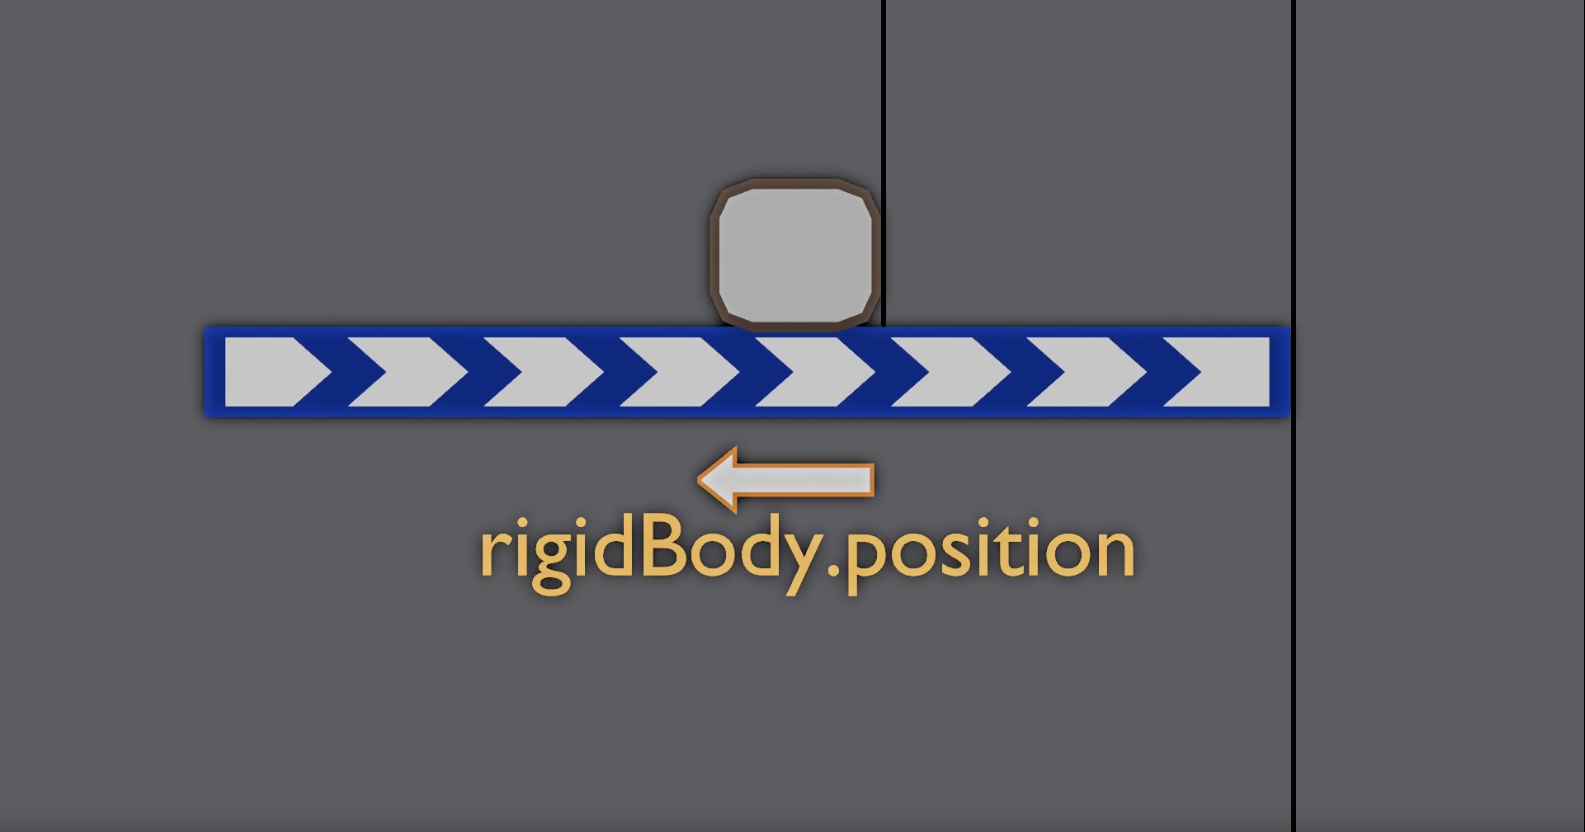
\includegraphics[width=10cm, height=6cm]{figures/rbodyposition1.png}
\caption{rigidBody Position 1}
\label{fig:rbodyposition1}
\end{figure}


En la Figura ~\ref{fig:rbodyposition1} se presenta el movimiento de la cinta, este movimiento solo aplica para la cinta, a diferencia del método MovePosition que se presenta más adelante.
\clearpage

\begin{figure}[h]
\centering
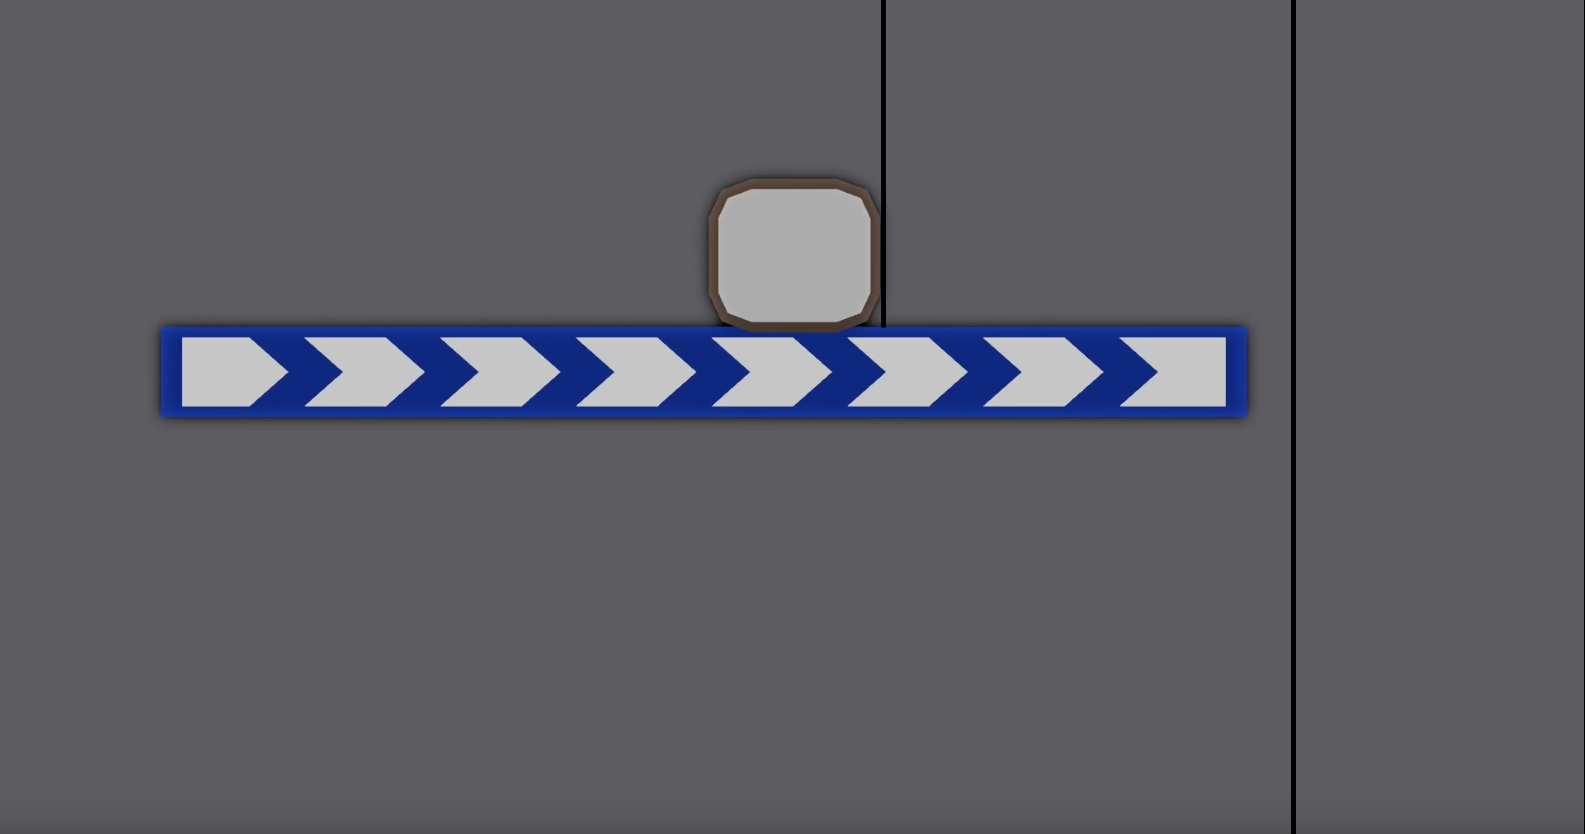
\includegraphics[width=10cm, height=6cm]{figures/rbodyposition2.png}
\caption{rigidBody Position 2}
\label{fig:rbodyposition2}
\end{figure}

En la Figura ~\ref{fig:rbodyposition2} se muestra donde finaliza el movimiento, como se aprecia este solo mueve la cinta y el objeto sobre esta no posee movimiento

\begin{lstlisting}[frame=single]
        rBody.MovePosition(pos);
\end{lstlisting}
En este método, se devuelve la cinta a su posición original, la diferencia que con el método de movimiento anterior es que si se mueve el objeto, tal como se presenta en las siguientes figuras.
\begin{figure}[h]
\centering
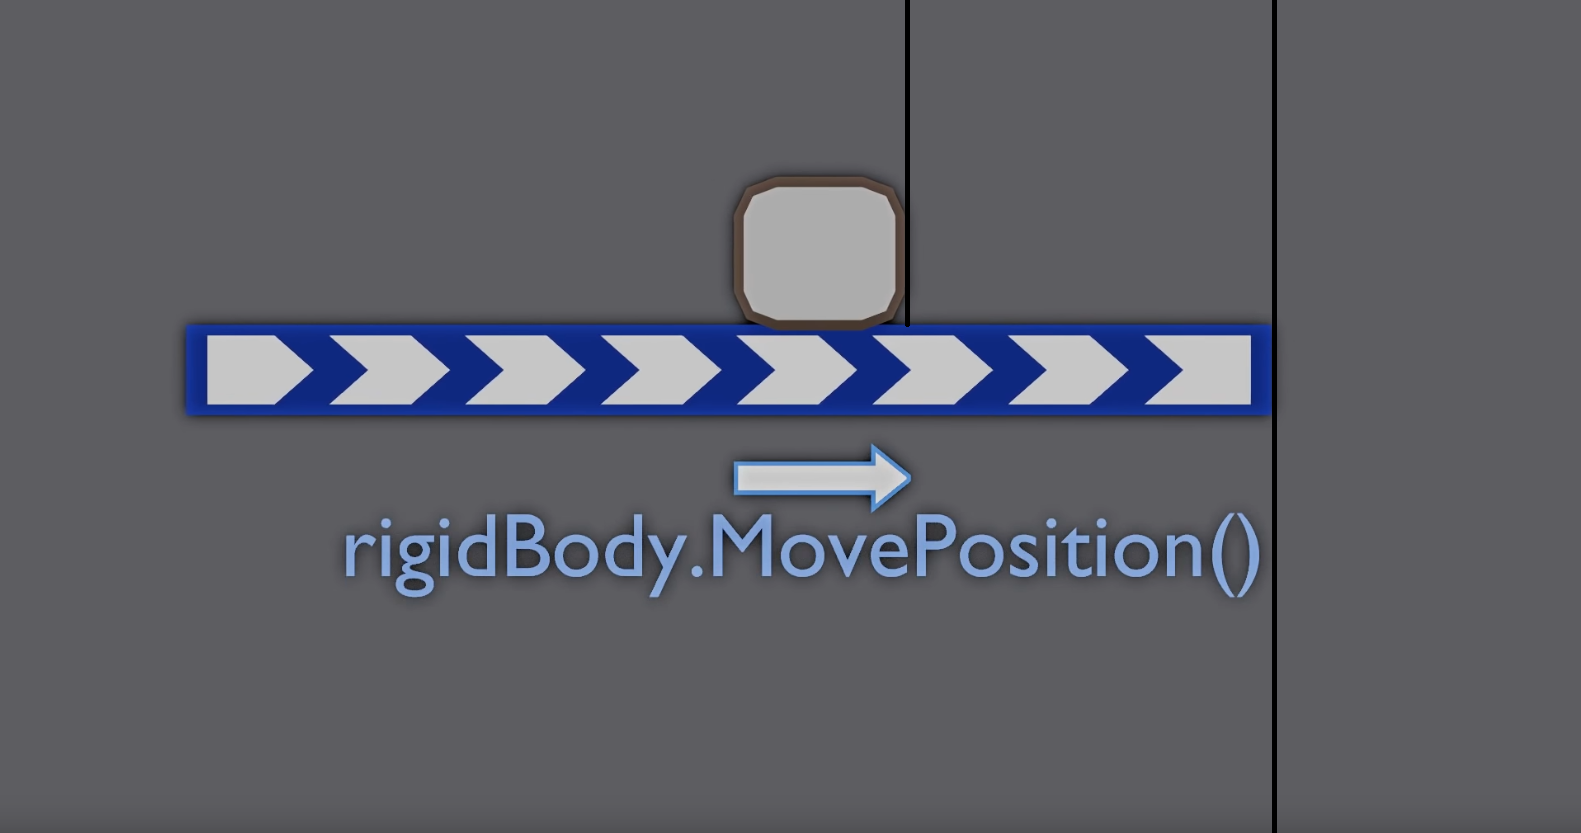
\includegraphics[width=10cm, height=6cm]{figures/rbodymove1.png}
\caption{rigidBody MovePosition 1}
\label{fig:rbodymove1}
\end{figure}

En la Figura ~\ref{fig:rbodymove1} se presenta el movimiento de la cinta, este movimiento aplica tanto para la cinta como para el objeto.

\clearpage

\begin{figure}[h]
\centering
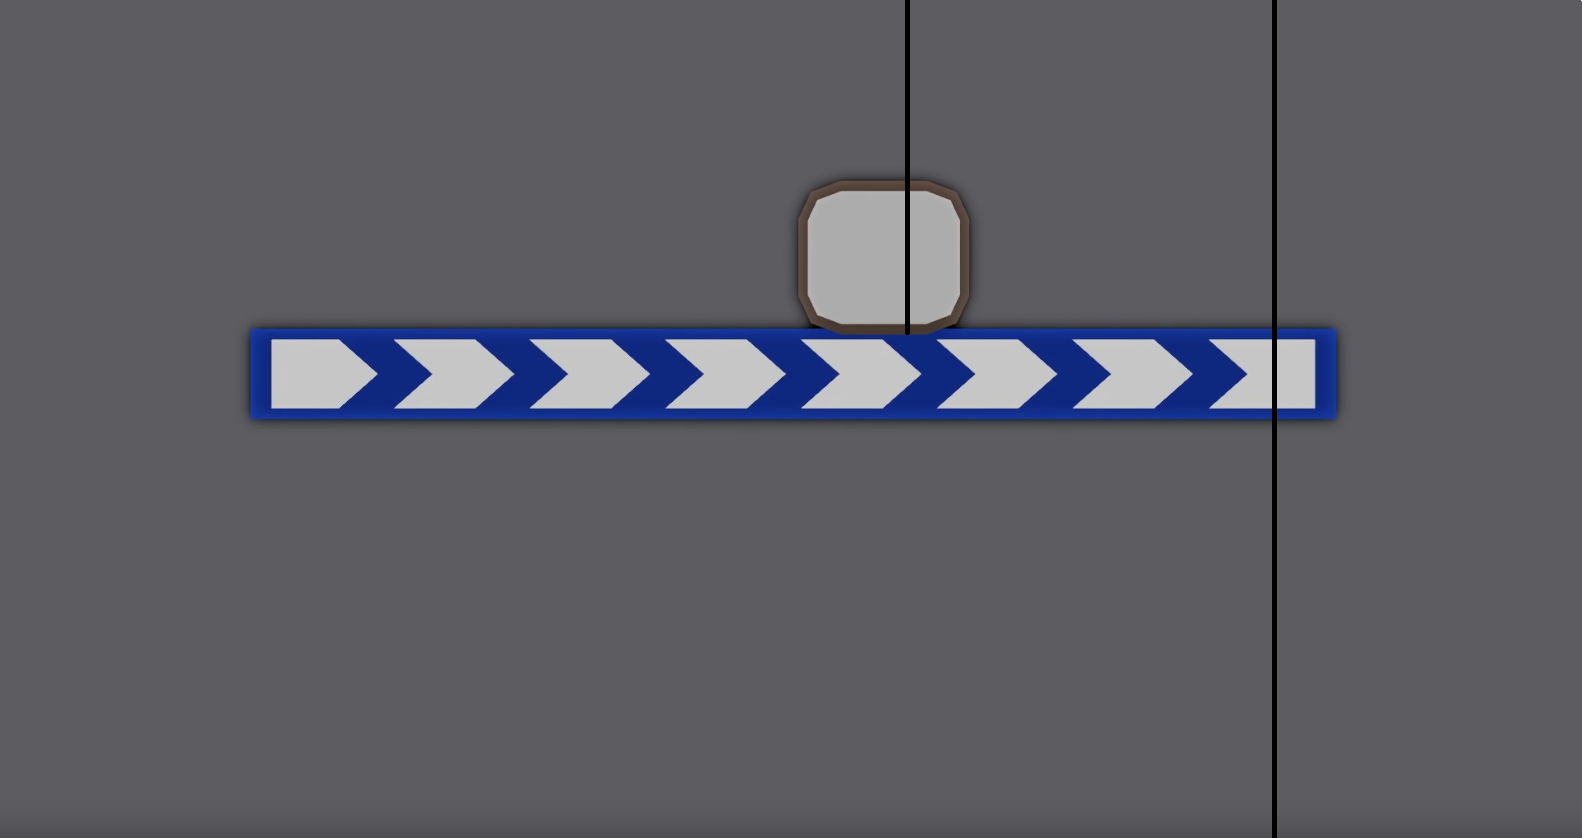
\includegraphics[width=10cm, height=6cm]{figures/rbodymove2.png}
\caption{rigidBody MovePosition 2}
\label{fig:rbodymove2}
\end{figure}

En la Figura ~\ref{fig:rbodymove2} se muestra donde finaliza el movimiento, como se aprecia este mueve tanto la cinta y como el objeto.

Con esta sucesión de movimientos, la cinta al "ir para atrás" sin mover el objeto, y después "volver a su posición" moviendo el objeto, repitiéndolo una y otra vez se logra el efecto de una cinta transportadora. El problema es que el objeto solo se mueve y en las esquinas no rota como en el laboratorio.
\clearpage
\section{Lógica Brazos Robóticos}
Para esta lógica, se explican los detalles mas importantes debido a que el código es demasiado extenso.
\begin{lstlisting}[frame=single]
   //Base
    public float velocidadRotacionBase = 50.0f; // Velocidad de rotacion
    public KeyCode teclaRotacionPositivaBase = KeyCode.Q; // Tecla para la rotacion en direccion positiva
    public KeyCode teclaRotacionNegativaBase = KeyCode.A; // Tecla para la rotacion en direccion negativa
    public Transform Base; // Transform del objeto que se va a rotar
    private float LimitePositivoBase = 155.0f; // Angulo limite del objeto
    private float LimiteNegativoBase = -155.0f; // Angulo limite del objeto
    private float sumaRotacionBase = 0.0f; // Suma de la rotacion del objeto para su uso en limites

    //Shoulder
    public float velocidadRotacionShoulder = 50.0f; // Velocidad de rotacion
    public KeyCode teclaRotacionPositivaShoulder = KeyCode.W; // Tecla para la rotacion en direccion positiva
    public KeyCode teclaRotacionNegativaShoulder = KeyCode.S; // Tecla para la rotacion en direccion negativa
    public Transform Shoulder; // Transform del objeto a rotar
    public Transform puntoFijoShoulder; // Transform del punto fijo alrededor del cual se realizara la rotacion
    private float LimitePositivoShoulder = 10.0f; // Angulo limite del objeto
    private float LimiteNegativoShoulder = -130.0f; // Angulo limite del objeto
    private float sumaRotacionShoulder = 0.0f; // Suma de la rotacion del objeto para su uso en limites
\end{lstlisting}
Para explicar las declaraciones de las partes de los brazos, se toma en cuenta dos partes distintas pero aplica para cualquier otra parte similar, la base es un objeto que tiene rotación sobre su propio eje, es decir no necesita otro punto para rotar o rota sobre su propio centro, a diferencia del Shoulder o un brazo cualquiera, para rotar este tiene un punto fijo en uno de sus extremos y no en el centro.
Se empieza con declarar la velocidad de la rotación del objeto en una variable float. Después se declaran variables tipo KeyCode que sirven para almacenar la información de una tecla en el teclado en particular, esto se realiza para realizar pruebas de movimiento.
Al declarar una variable de tipo Transform, en Unity, un "Transform" se refiere a un componente fundamental que se encuentra en la mayoría de los objetos en un escenario 3D o 2D. El componente Transform está asociado con la posición, rotación y escala de un objeto en el espacio de juego. Básicamente, controla la ubicación y la orientación de un objeto en el mundo virtual creado en Unity. Con esta variable se puede guardar toda la información previamente descrita, con la finalidad de realizar movimientos. En casos de rotación sobre el mismo objeto como la Base, solo se pide una variable, para objetos con centro en su extremo se piden dos variables, mas adelante se detallara como funciona el movimiento y el motivo de pedir uno o dos variables.
Y por ultimo se tienen los limites, consisten en dos variables que marcan el limite de operación de cada parte, para este caso se utilizan los limites establecidos mecánicamente por la misma unidad descrita en su manual. Y también la suma de rotación, la cual almacenara como tal el movimiento realizado, esto para ser utilizado en la comprobación de limites

\begin{lstlisting}[frame=single]
    private string nombreObjeto = "";
\end{lstlisting}
En esta linea se declara una variable para identificar la parte que se moverá con la botonera.

\begin{lstlisting}[frame=single]
    private bool positivoboton = false;
    private bool negativoboton = false;
\end{lstlisting}
Con estas variables sirven para saber si el botón presionado es positivo o negativo

\begin{lstlisting}[frame=single]
    private bool isControlPressed = false;
    private bool isAltPressed = false;
\end{lstlisting}
Para estas lineas se utilizo para realizar pruebas para guardar posiciones y realizar el movimiento a esa posición, estas servían para saber si Control fue presionado o el Alt fue presionado

\begin{lstlisting}[frame=single]
    private bool EmpezarGuardar = false;
    private bool TerminarGuardar = false;
    private bool EmpezarMover = false;
    private bool TerminarMover = false;
\end{lstlisting}
Acá los booleanos son para lo descrito anteriormente, sirven para marcar los inicios y finales de guardar posiciones y mover a las posiciones

\begin{lstlisting}[frame=single]
    private int NumeroUsar = -1;
\end{lstlisting}
Este numero es el numero usado en la botonera, en el cual se guardara la información.

\begin{lstlisting}[frame=single]
    private Dictionary<int, float> GuardarBase = new Dictionary<int, float>();
    private Dictionary<int, float> GuardarShoulder = new Dictionary<int, float>();
    private Dictionary<int, float> GuardarElbow = new Dictionary<int, float>();
    private Dictionary<int, float> GuardarWrist = new Dictionary<int, float>();
    private Dictionary<int, float> GuardarEndEffector = new Dictionary<int, float>();
\end{lstlisting}
Estas variables son diccionarios, los cuales con una variable devuelve una segunda variable, con esto poder guardar por ejemplo, la posición dependiendo del numero requerido, función que ocupa la botonera. Esta declarada para que con un numero entero devuelva un flotante.

\clearpage
\begin{lstlisting}[frame=single]
    private void Start()
    {
        GuardarBase.Add(0, 0f);
        GuardarShoulder.Add(0,0f);
        GuardarElbow.Add(0,0f);
        GuardarWrist.Add(0,0f);
        GuardarEndEffector.Add(0,0f);
    }
\end{lstlisting}
Al ejecutar el programa, en su inicio ejecutara esta secuencia de funciones, las cuales son para agregar la posición cero a los diccionarios.

\begin{lstlisting}[frame=single]
    private void Update()
    {
        Movimiento(Base, teclaRotacionPositivaBase, teclaRotacionNegativaBase, velocidadRotacionBase, LimitePositivoBase, LimiteNegativoBase, Base, Base.up, ref sumaRotacionBase);
        Movimiento(Shoulder, teclaRotacionPositivaShoulder, teclaRotacionNegativaShoulder, velocidadRotacionShoulder, LimitePositivoShoulder, LimiteNegativoShoulder, puntoFijoShoulder, puntoFijoShoulder.forward, ref sumaRotacionShoulder);
        Movimiento(Elbow, teclaRotacionPositivaElbow, teclaRotacionNegativaElbow, velocidadRotacionElbow, LimitePositivoElbow, LimiteNegativoElbow, puntoFijoElbow, puntoFijoElbow.forward, ref sumaRotacionElbow);
        Movimiento(Wrist, teclaRotacionPositivaWrist, teclaRotacionNegativaWrist, velocidadRotacionWrist, LimitePositivoWrist, LimiteNegativoWrist, puntoFijoWrist, Wrist.forward, ref sumaRotacionWrist);
        Movimiento(EndEffector, teclaRotacionPositivaEndEffector, teclaRotacionNegativaEndEffector, velocidadRotacionEndEffector, LimitePositivoEndEffector, LimiteNegativoEndEffector, puntoFijoEndEffector, EndEffector.right, ref sumaRotacionEndEffector);
        MovimientoBoton(nombreObjeto);
        Guardar();
        Usar();
        GuardarBoton();
        UsarBoton();
        MoverEje();
        MoverEjeBoton();
    }
\end{lstlisting}
El update se encarga de que el programa este esperando una interacción por parte del usuario para realizar una función, las cuales se explicaran a continuación.
\clearpage
\begin{lstlisting}[frame=single]
    private void Movimiento(Transform objeto, KeyCode TeclaPositiva, KeyCode TeclaNegativa, float VelocidadRotacion, float anguloLimitePositivo, float anguloLimiteNegativo, Transform puntoFijo, Vector3 direccion, ref float Suma)
    {
        float direccionRotacion = 0.0f;
        if (Input.GetKey(TeclaPositiva))
        {
            direccionRotacion = 1.0f;
        }
        else if (Input.GetKey(TeclaNegativa))
        {
            direccionRotacion = -1.0f;
        }
        if (direccionRotacion == 0.0f)
        {
            return;
        }
        float anguloRotacion = direccionRotacion * VelocidadRotacion * Time.deltaTime;
        float anguloRotacionLimitado = Mathf.Clamp(Suma, anguloLimiteNegativo, anguloLimitePositivo);
        if(anguloRotacionLimitado == anguloLimiteNegativo && direccionRotacion < 0)
        {
            anguloRotacion = 0.0f;
        }

        if(anguloRotacionLimitado == anguloLimitePositivo && direccionRotacion > 0)
        {
            anguloRotacion = 0.0f;
        }
        objeto.RotateAround(puntoFijo.position, direccion, anguloRotacion);
        Suma += anguloRotacion;
        Suma = Mathf.Clamp(Suma, anguloLimiteNegativo, anguloLimitePositivo);
    }
\end{lstlisting}
En la programación del simulador, lo principal fue realizar los movimientos de los brazos robóticos, los cuales principalmente se probaron mediante teclado y no por la botonera. Este código da origen al usado en la botonera, por lo que se explica el código de la botonera.
\clearpage
Para utilizar la botonera, primero se parte detectando que botón se esta presionando

\begin{lstlisting}[frame=single]
    public void PointerUpPositivo(string nombre)
    {
        nombreObjeto = nombre;
        positivoboton = false;
    }

    public void PointerDownPositivo(string nombre)
    {
        nombreObjeto = nombre;
        positivoboton = true;
        
    }

    public void PointerUpNegativo(string nombre)
    {
        nombreObjeto = nombre;
        negativoboton = false;
    }

    public void PointerDownNegativo(string nombre)
    {
        nombreObjeto = nombre;
        negativoboton = true;
    }
\end{lstlisting}
El método Pointer sirve para identificar los cambios de estado del puntero, ya sea que se haya ejecutado un clic o se mantenga presionado.
Con esto se puede pasar a la función de MovimientoBoton.

\begin{lstlisting}[frame=single]
    private void MovimientoBoton(string nombre)
    {
        float direccionRotacionboton = 0.0f;
        if (positivoboton)
        {
            direccionRotacionboton = 1.0f;
        }
        if (negativoboton)
        {
            direccionRotacionboton = -1.0f;
        }
        if (direccionRotacionboton == 0.0f)
        {
            return;
        }
\end{lstlisting}
Con el método anterior Pointer, se cambia el estado del booleano, el cual le da la direccion de movimiento.

\begin{lstlisting}[frame=single]
        float Sumar = 0;
        Vector3 direccion = Vector3.up;
        float anguloLimitePositivo = 0;
        float anguloLimiteNegativo = 0;
        float VelocidadRotacion = 0;
        Transform puntoFijo = Base;
        Transform objeto = Base;
\end{lstlisting}
Estos datos se pueden considerar como ''basura'', debido que estos se declaran solo para evitar el error nulo de Unity.

\begin{lstlisting}[frame=single]
        if (nombre == "Base")
        {
            Sumar = sumaRotacionBase;
            direccion = Base.up;
            anguloLimitePositivo = LimitePositivoBase;
            anguloLimiteNegativo = LimiteNegativoBase;
            VelocidadRotacion = velocidadRotacionBase;
            puntoFijo = Base;
            objeto = Base;
        }
\end{lstlisting}
En el método Pointer, este aparte de detectar un click, trae el nombre del botón presionado, con esto se reescribe los datos ''basura'' anteriormente declarados, para tener los datos que corresponden, esto para cada articulación del brazo.

\begin{lstlisting}[frame=single]
        float anguloRotacion = direccionRotacionboton * VelocidadRotacion * Time.deltaTime;
        float anguloRotacionLimitado = Mathf.Clamp(Sumar, anguloLimiteNegativo, anguloLimitePositivo);
\end{lstlisting}
En esta parte se ejecutan los cálculos de la rotacion, primero se adapta el movimiento a una velocidad que Unity pueda interpretar.
Después se realiza la comprobación de que la suma de movimiento (la cual representa el angulo que posee a partir de su punto inicial) se encuentre dentro de los limites establecidos.

\begin{lstlisting}[frame=single]
        if(anguloRotacionLimitado == anguloLimiteNegativo && direccionRotacionboton < 0)
        {
            anguloRotacion = 0.0f;
        }
        if(anguloRotacionLimitado == anguloLimitePositivo && direccionRotacionboton > 0)
        {
            anguloRotacion = 0.0f;
        }
\end{lstlisting}
Aca se utiliza una segunda comprobación, pues aunque se revisara antes si la suma se encontraba dentro de los limites, este no limitaba un movimiento, por el cual la articulación sigue el movimiento. Para evitar el movimiento se agrega comprobar si la suma(el anguloRotacionLimitado es igual a la suma) es igual a los limites, y de ser asi, este elimina el anguloRotacion, eliminando cualquier movimiento calculado.

\begin{lstlisting}[frame=single]
        objeto.RotateAround(puntoFijo.position, direccion, anguloRotacion);
\end{lstlisting}
El método RotateAround se encarga de realizar el movimiento de las articulaciones, se elige este método al ser mas ''universal'' y el código final fue compatible con diferentes modelos sin tener que realizar modificaciones a este.

\begin{lstlisting}[frame=single]
        Sumar += anguloRotacion;
        Sumar = Mathf.Clamp(Sumar, anguloLimiteNegativo, anguloLimitePositivo);
\end{lstlisting}
Para ir finalizando, se agrega el angulo recién operado a la suma, ademas de comparar si este se sale o no de su limite, esto debido que internamente en Unity se iban agregando decimales, aunque sean de muy poco valor, estos al sumar llegarían a alterar los ángulos

\begin{lstlisting}[frame=single]
        if (nombre == "Base")
        {
            sumaRotacionBase = Sumar;
        }
    }
\end{lstlisting}
Y por ultimo, se guarda la suma en su variable correspondiente.

\clearpage
\section{Lógica tomar objeto}

\begin{lstlisting}[frame=single]
    public void OnClick()
    {
        if(podertomar)
        {
            boton = true;
        }
        if(tomado)
        {
            boton = false;
        }
        
    }
\end{lstlisting}
Aca se espera un Click en el botón, verificando si el booleano podertomar es verdadero para activar la función del botón, caso contrario se revisa si el booleano tomado es verdadero para desactivar la función del botón

\begin{lstlisting}[frame=single]
    private void OnTriggerStay(Collider other)
    {
        if(other.gameObject.CompareTag("Objeto"))
        {
            if(pickedObject == null)
            {
                podertomar = true;
                if(Input.GetKey("z") || boton)
                {
                    other.GetComponent<Rigidbody>().useGravity = false;
                    other.GetComponent<Rigidbody>().isKinematic = true;
                    other.transform.position = handPoint.transform.position;
                    other.gameObject.transform.SetParent(handPoint.gameObject.transform);
                    pickedObject = other.gameObject;
                    tomado = true;
                    podertomar = false;
                    boton = true;
                }
            }
        }
    }
\end{lstlisting}
El método OnTriggerStay sirve cuando dos objetos en Unity colisionan, con esto se compara que el objeto colisionado tiene la etiqueta de ''Objeto''.
Después se revisa que no exista un objeto ya tomado, al ser nulo, este activa la función de podertomar.
El objeto al estar tomado, se le desactivan la función de gravedad para poder mantenerse en la posición designada, dando el efecto de agarre.
También se le activa la propiedad de kinemático, el cual hace que el objeto no se vea afectado por fuerzas externas o colisiones.
Después se le asigna la posición de ''mano'', la cual al desarrollarlo se debe establecer, y por ultimo agrega el objeto como ''hijo'', con esto seguirá el movimiento del robot

\begin{lstlisting}[frame=single]
    void Update()
    {
        if(pickedObject != null)
        {
            if(Input.GetKey("x") || !boton)
            {
                pickedObject.GetComponent<Rigidbody>().useGravity = true;
                pickedObject.GetComponent<Rigidbody>().isKinematic = false;
                pickedObject.gameObject.transform.SetParent(null);
                pickedObject = null;
                tomado = false;
            }
            
        }
    }
\end{lstlisting}

En esta parte se suelta el objeto, cambiando las propiedades anteriormente modificadas, eliminando el parentesco, y nuevamente dejando el brazo listo para poder tomar otro objeto.